\documentclass[11pt]{article}

\usepackage{amsmath}
\usepackage{textcomp}
\usepackage{graphicx}

\usepackage[top=0.8in, bottom=0.8in, left=0.8in, right=0.8in]{geometry}
\usepackage{listings}
\usepackage{color}

\definecolor{dkgreen}{rgb}{0,0.6,0}
\definecolor{gray}{rgb}{0.5,0.5,0.5}
\definecolor{mauve}{rgb}{0.58,0,0.82}

\lstset{frame=tb,
  language=Java,
  aboveskip=3mm,
  belowskip=3mm,
  showstringspaces=false,
  columns=flexible,
  basicstyle={\small\ttfamily},
  numbers=none,
  numberstyle=\tiny\color{gray},
  keywordstyle=\color{blue},
  commentstyle=\color{dkgreen},
  stringstyle=\color{mauve},
  breaklines=true,
  breakatwhitespace=true,
  tabsize=3
}

% Add other packages here %


% Put your group number and names in the author field %
\title{\bf Excercise 3\\ Implementing a deliberative Agent}
\author{Group \textnumero 15: Student 1, Student 2}


% N.B.: The report should not be longer than 3 pages %


\begin{document}
\maketitle

\section{Model Description}

\subsection{Intermediate States}
% Describe the state representation %
In our model we have decided to represent our States with the following attributes:

\begin{lstlisting}
		private int availableCapacity; // stores available capacityof the vehicle in the specific state
    	private City currentCity; // stores the current city where the vehicle is located in the specific state 
    	private List<Task> availableTasks; // list of tasks available in the topology, ie tasks not yet taken by the vehicle in the state being considered.
    	private List<Task> carriedTasks; // list of states taken by the agent but not yet delivered
\end{lstlisting}We opted for this model as it resulted to be more than enough for the state-based search and the reconstruction of the optimum plan.


\subsection{Goal State}
% Describe the goal state %
Goal States are simply all those states that have both empty the "availableTasks" and "carryTasks" lists.

\subsection{Actions}
% Describe the possible actions/transitions in your model %
To describe the evolution of our model from a current state to the next state we were based on the simple choice that the agent moves to a neighbour city of the current city. Therefore, for each neighbour city of the current city there will be a next state that is built as follows:
\begin{enumerate}
\item It is checked if in the neighbour city we can deliver tasks between our carriedTasks, in the positive case we update the list of carriedTasks and the availableCapacity.
\item Consequently, we check if in the neighbour city there are tasks that can be taken (considering our availableCapacity), if so, we update the lists "availableTasks" and "carriedTasks" and the availableCapacity.
\end{enumerate}When this is done, the next state in the neighbour city is initialized.
\\
This procedure is repeated for each neighbour city of the current city, and it is used in a method called "getAllNodeChildren (currentNode)" that returns all of the next possible children nodes of the current node.

\section{Implementation}

\subsection {Node class}
For the implementation of the two search algorithms we have modeled a Node class so we can reconstruct the best path at the end of the research. The class contains the following attributes:
\begin{lstlisting}
    private State state; // stores the current state examined
    private Node father; // stores the father Node of this node
    private double finalCost; // stores the final cost of the state for the A* algorithm
    private double distanceCost; // stores the distance cost of the current state
    private double heuristicCost; // stores the heuristic cost of the current state
\end{lstlisting}Once the research has been completed, the path is reconstructed recursively in the "createPath" method and finally the actions for the optimum plan are created with the help of the "createActions (State currentState, State NextState)" method that returns a list of Logist actions needed to get to the nextState.

\subsection{BFS}
% Details of the BFS implementation %
The implementation of the BFS follows what was presented during lessons with a slight change, ie when a Goal State (a leaf) is found, it is checked if the "distanceCost" of the current node is less than the distanceCost of the best goalNode found earlier, in the positive case the new goalNode becomes the best current GoalNode. This is because in this specific problem we are forced to find all the goals State and then decide which one is the best.
\\
To verify whether a State has already been visited (that is, it is contained in the set of states already visited) we override the equals method for the State class. Finally, as mentioned above, we have defined the "getAllChildren (currentState)" method for obtaining child states in the current state, which is described in the previous paragraph.

\subsection{A*}
% Details of the A* implementation %
For the implemantation of the A* we used a PriorityQueue to store the all the nodes that are created but that haven't been visited yet. The Priority Queue uses a Comparator in order to store the nodes following an ascending order of the total cost. The total cost of a node, that we can see as f(n) = g(n) + h(n), is composed of two factors: the cost from the root to that node (g(n)) and the heuristic of that node (h(n)), that calculate a prevision of the cost from that node to the node containing the goal state.\\
The first step is to add in the queue the root. After that we enter in a loop that stops only if the queue is empty or if a goal state is found. The loop is described as follows:
\\
\\
We take the first node in the queue (from now on called notVisitedQueue), and we get the state inside. If it is a goal state, we recreate the path using the function "createPath(currentNode)" and we exit the loop. Otherwise, if the node has not already been visited, we add it to the nodesVisitedList.\\
Now we work on the children of the node, obtained through the "getAllChildren(currentNode)" method: for every child, if it is not contained in the nodesVisitedList (remember: a node has already been visited if the currentState inside has already been seen by the algorithm) and is not contained in the notVisitedQueue, we add it to the last one (it will be in the right order because it is a Priority Queue). If it is contained in the nodesVisited list, two things can happen: if the g(n) of this node we are working on is lower than the one saved in the list, we remove the node from the nodesVisitedList because it means that we have found a better path for that node, otherwise we do nothing.

\subsection{Heuristic Function}
% Details of the heuristic functions: main idea, optimality, admissibility %
We defined two different heuristic functions for the A* algorithm. We will go through their differences and we will make experiments in order to show them.
\\
We will refer to different costs in the next sections.\\
The cost to go from a city \textit{Cx} to a city \textit{Cy} is given by the following formula:
\begin{equation}
c(Cx, Cy) = d(Cx, Cy) * costPerKm
\end{equation}where \textit{c} is the cost function, \textit{d} is the distance between the two cities following the shortest path and \textit{costPerKm} is the cost per kilometer of the vehicle.\\
When we compute the \textbf{cost of a current task} \textit{Tc} we will use the following formula:
\begin{equation}
c(Tc) = d(Cc, Cd) * costPerKm
\end{equation}where \textit{c} is the cost function, \textit{d} is the distance between two cities as above, and \textit{Cc} and \textit{Cd} are respectively the current city of the agent and the city where the task \textit{T} has to be delivered.\\
\\
When we compute the \textbf{cost of an available task} \textit{Ta} we will use the following formula:
\begin{equation}
c(Ta) = (d(Cc, Cp) + d(Cp, Cd)) * costPerKm
\end{equation}where \textit{c}, \textit{d}, \textit{Cc}, \textit{Cd} are as defined above and \textit{Cp} is the city where the task as to be picked up.

\subsubsection{First Heuristic Function}

We tried a first heuristic function that considered only the costs of tasks containing cities that were not contained in any other task. We were sure that we were not overstimating the actual cost because we were summing only a part or at most all the actual costs, no more. We noticed that often the heuristic was returning 0, because every task present had some city contained in other tasks. For this reason we thought about another possible solution, that is the next heuristic function described.

\subsubsection{Second Heuristic Function}

The second heuristic function is defined as follows: "Given a set of available tasks \textit{AT} and a set of current tasks \textit{CT} in a state \textit{s}, the heuristic function for \textit{s} returns the maximum cost between all the present tasks in \textit{s}."\\

\textbf{Optimality:}\\
We are sure that we are not overstimating the actual cost because we are considering only the longest path that the agent will do. If there is only one task present, the heuristic function will return the exact cost from the current state to the goal state. If there are more, it will return a lower cost.

\section{Results}

\subsection{Experiment 1: BFS and A* Comparison}
% Compare the two algorithms in terms of: optimality, efficiency, limitations %
% Report the number of tasks for which you can build a plan in less than one minute %

After implementing both algorithms, we arrived at the expected conclusion: A* alghoritm is much faster (in terms of iterations) than BFS. As we saw a drastical decrease of number of iterations we have also noticed that the computational time increases as well. That happens probably because implementing A* in a Java environment could cause bottlenecks that increase the time of each iteration of the algorithm. However we didn't pursued the optimization of the computational time of the algorithm because we focused on the main problems of the assignment.

\subsubsection{Setting}
% Describe the settings of your experiment: topology, task configuration, etc. %
1) Topology: Switzerland topology; 2) Tasks: from 6 to 16 initial tasks

\subsubsection{Observations}
% Describe the experimental results and the conclusions you inferred from these results %
We compared the performances of the two algorithms. As you can see on the bar chart below, the A* is algorithm has better perfomances than the BFS. The only problem is that with 10 or more task the A* algorithm takes more than one minute to finish its loop (the BFS can manage 16 tasks under one minute). For this reason we didn't reported the perfomances of the A* with 11 tasks or more. As expected final rewards per Km for both algorithms are the same because both of them find the optimal plan. In particular, for a number of tasks of 7, 8 and 9 we have respectively 200 reward/Km, 230 reward/Km, 270 reward/Km.\\
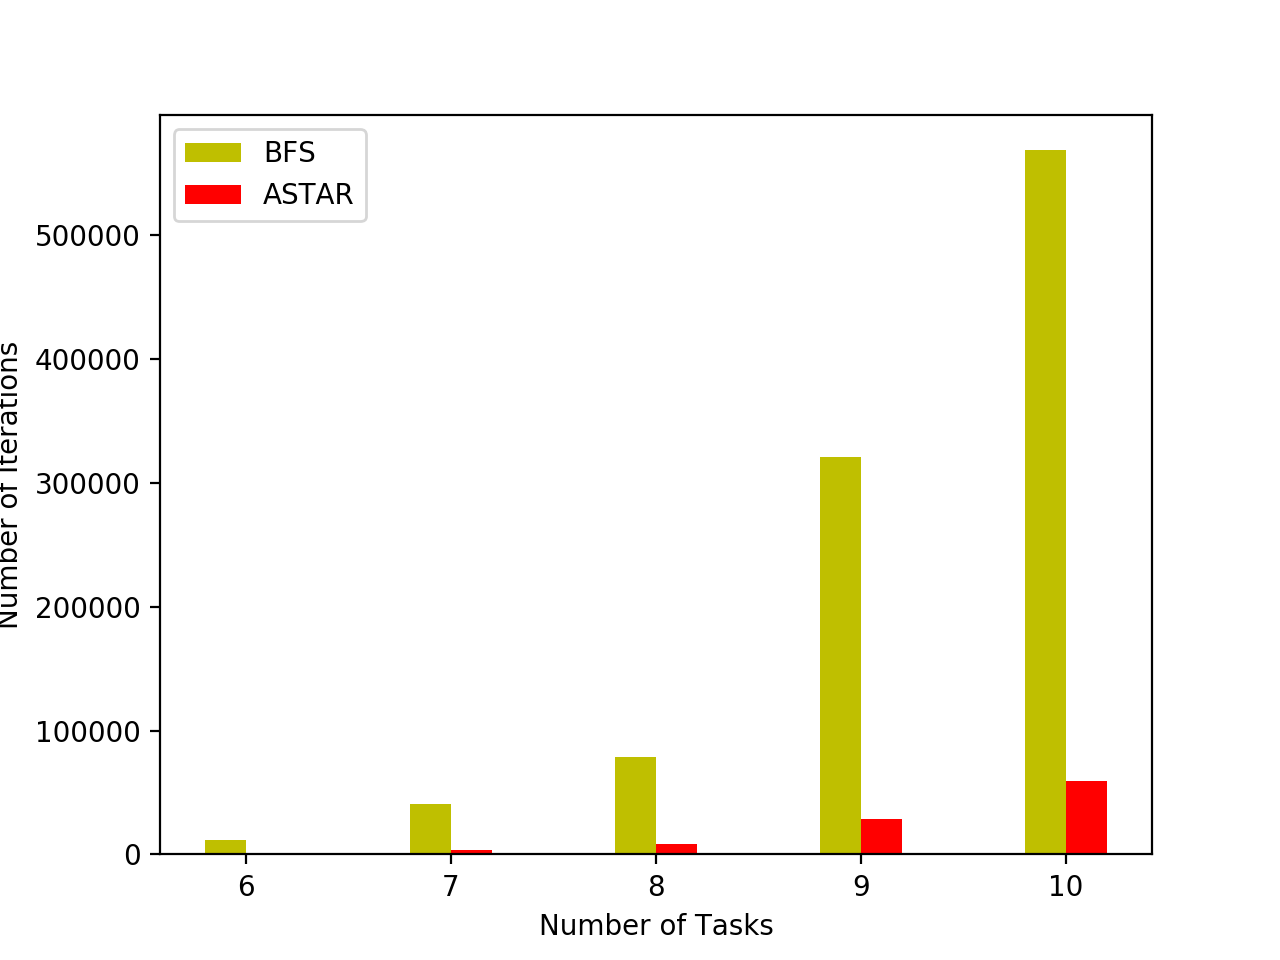
\includegraphics[scale=0.5]{bar.png}
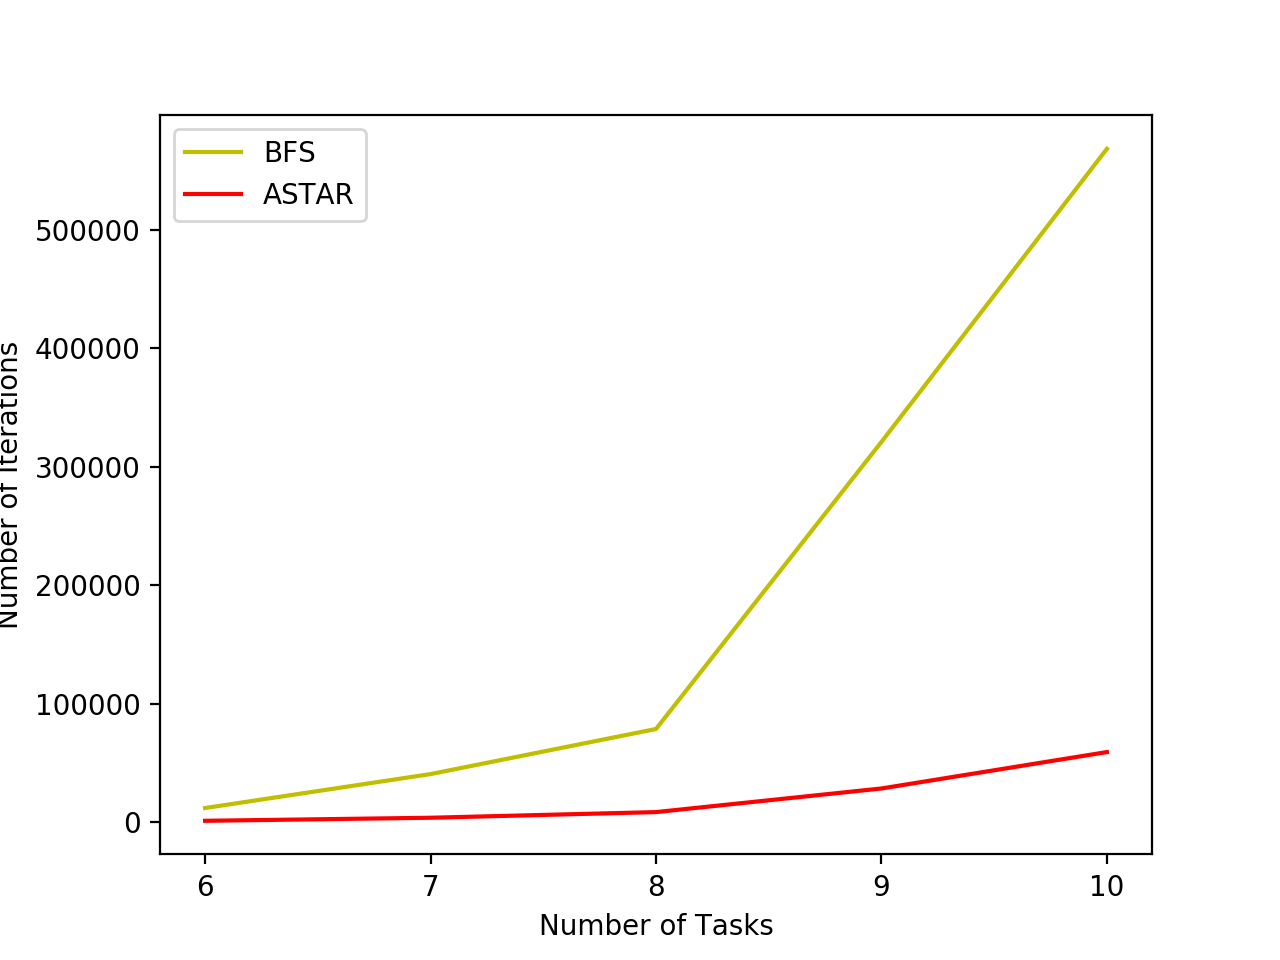
\includegraphics[scale=0.5]{plot.png}



\subsection{Experiment 2: Multi-agent Experiments}
% Observations in multi-agent experiments %

\subsubsection{Setting}
% Describe the settings of your experiment: topology, task configuration, etc. %

\textbf{First Experiment}: Available Tasks = 8; Three Agents = BFS, BFS, BFS
\\
\\
\textbf{Second Experiment}: Available Tasks = 8; Three Agents = A*, BFS, BFS
\subsubsection{Observations}
% Describe the experimental results and the conclusions you inferred from these results %
\textbf{First Experiment}:\\
When all the agents use the same algorithm, the only factor that counts for the final rewards is where they start. The logist platform doesn't create the three agents in the same moment, but one after the other. In conclusion, we can say that who was born as first and in a better city to start will be the agent with the best plan and will have a greater probability of stealing the tasks to all the others.\\
\\
\textbf{Second Experiment}:\\
As already said, we can't really infer a lot about these experiments because the result depends on the order the agents are created and where they were born. The plan they find, even if they use A* or BFS, is always the optimal plan.



\end{document}